% Opcje klasy 'iithesis' opisane sa w komentarzach w pliku klasy. Za ich pomoca
% ustawia sie przede wszystkim jezyk i rodzaj (lic/inz/mgr) pracy, oraz czy na
% drugiej stronie pracy ma byc skladany wzor oswiadczenia o autorskim wykonaniu.

\documentclass[declaration,shortabstract, mgr]{iithesis}
\usepackage{graphicx}
\usepackage[utf8]{inputenc}

%%%%% DANE DO STRONY TYTUłOWEJ
% Niezaleznie od jezyka pracy wybranego w opcjach klasy, tytul i streszczenie
% pracy nalezy podac zarowno w jezyku polskim, jak i angielskim.
% Pamietaj o madrym (zgodnym z logicznym rozbiorem zdania oraz estetyka) recznym
% zlamaniu wierszy w temacie pracy, zwlaszcza tego w jezyku pracy. Uzyj do tego
% polecenia \fmlinebreak.
\polishtitle {System kontroli obecności na podstawie elektronicznych legitymacji studenckich}
\englishtitle {Students attendence verifing system with the use of student card}
\polishabstract {\ldots}
\englishabstract{\ldots}
% w pracach wielu autorow nazwiska mozna oddzielic poleceniem \and
\author {Dawid Szczyrk}
% w przypadku kilku promotorow, lub koniecznosci podania ich afiliacji, linie
% w ponizszym poleceniu mozna zlamac poleceniem \fmlinebreak
\advisor {dr Jakub Michaliszyn}
%\date {} % Data zlozenia pracy
% Dane do oswiadczenia o autorskim wykonaniu
%\transcriptnum {} % Numer indeksu
%\advisorgen {dr. Jana Kowalskiego} % Nazwisko promotora w dopelniaczu
%%%%%

%%%%% WLASNE DODATKOWE PAKIETY
%
%\usepackage{graphicx,listings,amsmath,amssymb,amsthm,amsfonts,tikz}
%
%%%%% WłaASNE DEFINICJE I POLECENIA
%
%\theoremstyle{definition} \newtheorem{definition}{Definition}[chapter]
%\theoremstyle{remark} \newtheorem{remark}[definition]{Observation}
%\theoremstyle{plain} \newtheorem{theorem}[definition]{Theorem}
%\theoremstyle{plain} \newtheorem{lemma}[definition]{Lemma}
%\renewcommand \qedsymbol {\ensuremath{\square}}
% ...
%%%%%

\begin{document}

\chapter{Wprowadzenie}

Celem niniejszej pracy jest zaprojektowanie użytecznego i niedrogiego w utrzymaniu systemu do kontroli obecności studentów na wykładzie.\\
\indent Niemalże każde zajęcia na naszym instytucie zaczynają się od zebrania listy obecności. Odbywa się to w siermiężny sposób, ponieważ każdy ze studentów musi wpisać swoje dane na listę obecności.
Taka forma jest uciążliwa, zajmuje kilka pierwszych minut zajęć, a studenci się rozpraszają podając sobie listę obecności. Dziś, kiedy do ochrony danych osobowych przykłada się
coraz większą wagę, starodawne sposoby sprawdzania obecności są tym bardziej wątpliwe.\\
\indent W dobie współczesnych zdobyczy technologicznych można uznać za zaskakujące, że wziąć trafamy przy tym czasochłonnym procesie. Wydawać by się mogło, że obecne podejście jest tak zakorzenione w akademickiej kulturze, że nie ma możliwości tego zmienić. W niniejszej pracy chciałbym podjąć tę rękawicę i spróbować zaproponować rozwiązania które mogłyby cały proces znacznie usprawnić. \\
\indent Poniższa praca przedstawia proces od postawienia wymagań do realizacji finalnej wersji wielokomponentowego projektu. Na efekt ostateczny składają się aplikacje wykorzystujące najnowsze technologie i oparte na popularnych frameworkach, oraz niskopoziomowe elektroniczne urządzenie zaprojektowane i wykonane na potrzyby tego projektu.\\
\indent Z jednej strony ramach pracy musiałem zaprojektować komunikacje pomiędzy poszczególnymi komponentami, zaproponować i wdrożyć architekturę aplikacji internetowych, tzn. serwery na któych wykonywany jest kod stron internetowych oraz bazy danych. W wersji finalnej użytkownikowi umożliwiono stworzenie własnego konta w internetowym serwisie i zarządzanie danymi o obecnościach w jego kontekście. Wszystko to zostało oparte na nowoczesnych rozwiązaniach chmurowych. \\
\indent Z drugiej strony moim zadaniem było zaprojektowanie niedrogiego urządzenia elektronicznego, które miało za zadanie udostępniać zrozumiały interfejs i realizować zadania zwiazane ze zbieraniem danych od uczesników wykładu. Zagadnienie to wymagało wiedzy z zakresu elekroniki i zapoznania się ze schamatami połączeń pomiędzy poszczególnymi modułami i zrozumienia zasady ich działania. Dodatkowo ważnym elementem było połączenie odrępnych komponentów w jedną całość, a więc projekt układu elektronicznego na płytce stykowej i zamknięcie wszystkiego w opakowaniu umożliwiającym bezpieczne i wygodne użytkowanie. 


\chapter{Określenie wymagań}
\section{Analiza obecnego sposobu sprawdzania obecności}
W celu doprecyzowania wymagań stawianych przed projektowanym przeze mnie system postanowiłem rozważyć znany mi z autopsji proces weryfikowania obecności uczestników zajęć na zajęciach prowadzonych przez Uniwersytet Wrocławski\\
\indent Sprawdzanie listy obecności jest w dużej mierze uzależnione od preferencji prowadzącego i zwyczajów panujących na konkretnym wydziale - przykładowo obecność może być potwierdzona słownie - poprzez kolejne wywołanie osób z listy, albo pisemnie - poprzez udostępnienie listy na którą uczestnicy będą zobowiązani się wpisać.\\
\indent Dla uproszczenia dalszych rozważań postanowiłem przyjąć za ogólnie stosowaną metodę pisemną - która według moich obserwacji jest stosowana częściej - i na tej podstawie wyodrębnić czynności które składają się na wypełnienie listy obecności podczas zajęć.\\
\indent Zbieranie informacji o obecności studentów na wykładzie jest czynnością na pierwszy rzut oka oczywistą, po bliższym przyjrzeniu się całej procedurze, okazuje się jednak, że daje się ona rozłożyć na jeszcze prostsze elementy. \\

\begin{itemize}
\item Przygotowanie kartki z listą obecności (przypisanie listy obecności do zajęć których będzie ona dotyczyła).
\item Udostępnienie kartki uczestnikom oraz wpisywanie się na listę.
\item Weryfikacja poprawności zebranej listy poprzez przeliczenie osób obecnych na zajęciach.
\item Przeniesienie zebranych danych do uczelnianego systemu.
\end{itemize}

\indent Powyższy schemat zbierania listy obecności podatny jest na dodatkowe błędy. Nie trudno wyobrazić sobie sytuację w której student intencjonalnie podaje nie swoje dane w celu zaliczenia obecności innej osobie. Kolejnym krokiem który może doprowadzić do błędów na ostatecznej liście obecności jest błąd ludzki podczas przenoszenia danych z kartki do uczelnianego systemu komputerowego. Podobny błąd trudno jest od razu wychwycić ze względu na to, że studenci zazwyczaj nie przeglądają na bieżąco list obecności dostępnych np. na usosie. Kiedy na koniec semestru obecność jest rozliczana bardzo trudno dojść do faktów.\\
\indent Pierwszym elementem nadającym się w moim mniemaniu do usprawnienia jest samo tworzenie listy obecności z informację na temat zajęć których taka lista będzie dotyczyła. Fizyczna lista, poza czasem poświęconym na jej stworzenie musi być po odbytych zajęciach przechowywana - co stwarza ryzyko jej zgubienia. Dodatkowo istnieje prawdopodobieństwo, że trafi w niepowołane ręce i ktoś nieżyczliwy wpisze na nią dodatkowe nazwiska. Do tego wszystkiego dochodzi jeszcze aspekt ekologiczny, ponieważ każda kolejna kartka to dodatkowy element wyrwany matce naturze. \\
\indent Również udział studentów w rejestrowaniu własnej obecności może ulec optymalizacji. Wpisanie własnego imienia i nazwiska, a czasem numeru albumu zabiera czas, naraża na upublicznienie dane osobowe i utrudnia studentowi śledzenie wykładu.\\
\indent Weryfikacja poprawności listy jest nie tylko pracochłonna, ale również podatna na błędy. Czas poświęcony na policzenie uczestników rośnie wprost proporcjonalnie do ich liczby. Dodatkowo prowadzący zajęcia może się zwyczajnie pomylić albo ktoś dopisać do listy już po tym sprawdzeniu.\\
\indent Z całą pewnością usprawnienia wymaga proces przenoszenia danych z fizycznego nośnika do uczelnianego systemu komputerowego. Problemem jest nie tylko to, że podczas wpisywania obecności do komputerowego systemu można poopełnić błąd, ale również to, że jest to proces czasochłonny.\\

\section{Zdefiniowanie wymagań}

\indent Na podstawie poszczególnych kroków w procesie zbierania obecności, wyodrębniłem cztery właściwości przez pryzmat których mogłem ocenić potencjalne rozwiązania. Dodatkowo w dalszych rozważaniach do grona kryteriów oceny poszczególnych możliwości dołącze jeszcze dwa istotne elementy - przewidywany koszt, oraz stopień skomplikowania rozwiązania.

\subsection{Identyfikacja zajęć na których obecność była weryfikowana}
Jestem w stanie zidentyfikować dwa możliwe podejścia do tego problemu. Rozwiązanie tradycyjne realizuje to zadanie w naturalnej kolejności tzn. w momencie zbierania obecności wiemy dla jakich zajęć jest ona zbierana. W moim przekonaniu warto rozważyć opcję odwrotną, tzn. najpierw zbierać dane (pamiętając jedynie kiedy zostały zebrane), a w dalszej kolejności decydować jakich zajęć one dotyczą. W ten sposób unikamy konieczności wprowadzenia do nośnika informacji na temat tego jakich zajęć dotyczą zebrane dane.
\subsection{Zbieranie danych od studentów}
W tej kwestii brałem pod uwagę trzy możliwości. Tradycyjne rozwiązanie realizowane poprzez wpisywanie się na listę może zostać zastąpione poprzez użycie bardziej nowoczesnego sposobu identyfikacji - np. wbudowaną funkcję legitymacji studenckiej tj. identyfikację zbliżeniową. Innym sposobem byłoby zastąpienie fizycznej kartki wypełnianej przez osoby uczesniczące w zajęciach cyfrowym formularzem udostępnianym przez internetową aplikację. Ostatnią rozważaną przeze mnie możliwością jest skorzystanie z istniejącego albo stworzenie własnego systemu do rozpoznawania twarzy.
\subsection{Wprowadzenie danych do systemu}
To zadanie może być realizowane na dwa sposoby. Pierwszym z nich jest rejestrowanie obecności w systemie od razu przy jej odnotowaniu. W tym wypadku wymagane jest bezpośrednie połączenie z systemem. Drugim - zebranie wszystkich danych na wstępie i późniejsze, zbiorcze wprowadzanie ich do aplikacji. W tym wypadku niezbędny będzie nośnik na którym dane zostaną przetransportowane, wskazane jest również zaszyfrowanie tych danych na czas transportu.
\subsection{Weryfikacja poprawności danych}
W przypadku tradycyjnego zbierania obecności weryfikacja jest niedoskonała, ale konieczna ze względu na to że nośnik danych - kartka z listą obecności - udostępniana jest szerokiej publiczności. Podobny problem będzie występował jeśli kartkę papieru zastąpimy cyfrowym tabletem. Możemy również odseparować medium i każdą zebraną obecność weryfikować osobno.

\indent W kontekście powyższych rozważań zdecydowałem się na następujące założenia
\begin{itemize}
\item Implementowany przeze mnie system powinien być w stanie zbierać obecności bez wcześniejszego określenia w kontekście jakich zajęć jest to robione.
\item Dane od studentów powinny być zbierane bez ingerencji wykładowcy i nie zaburzając porządku zajęć.
\item Wprowadzanie danych powinno odbywać się w taki sposób, żeby uniknąć pomyłki.
\item Student nie powinien mieć możliwości ingerencji w listę obecności.
\end{itemize}

\section{Inne brane pod uwagę realizacje realizacje}
\subsection{Responsywna aplikacja internetowa umożliwiająca wygodne rejestrowanie obecności studentów na zajęciach w samej aplikacji przez internet albo telefon}. \\
W mojej ocenie to najprostsze rozwiązanie składające się z jednolitego systemu, w którym jednocześnie można zbierać obecności uczestników wykładu, oraz je przechowywać i przeglądać. Jej niewątpliwym plusem jest całkowite wyeliminowanie problemu związanego z wprowadzaniem danych do systemu katalogującego obecności, ponieważ dane wprowadzane są wprost do systemu. Identyfikacja konkretnych zajęć w ramach których rejestrowana jest obecność, odbywałaby się na początku zajęć poprzez wejście w kontekst opowiedniego wykładu w aplikacji. Obecność uczestników na zajęciach byłaby sprawdzana przez prowadzącego i od razu wprowadzana do systemu. \\
\indent Nie zdecydowałem się na to rozwiązanie, ponieważ wydaje mi się ono nieszczególnie odbiegać od aktualnej procedury, poza zminą nośnika z kartki papieru na ekran telefonu.
\subsection{Urządzenie rejestrujące obecności za pośrednictwem sieci bezprzewodowej}
To rozwiązanie początkowo wydało mi się bardzo atrakcyjne i przez długi czas miałem zamiar je zrealizować. Planowałem rozszerzyć mikrokontroler o moduł do bezprzewodowej łączności z internetem i w stworzonej aplikacji udostępnić interfejs do odnotowywania obecności. \\
\indent Po dłuższych rozważaniach okazało się jednak, że takie rozwiązanie przerasta moje możliwości. Ten sposób wysyłania danych do aplikacji katalogującej obecności  wymagałby umożliwienia powiązania obecności z zajęciami na których zostały zebrane \\
\indent Wymagałoby to dołączenia dodatkowego interfejsu który pozwalałby wprowadzać takie dane, co jeszcze bardziej komplikowałoby projektowane przeze mnie urządzenie. Dodatkowo ogtraniczyłoby to zbiór układów scalonych z których mógłbym skorzystać, ponieważ musiałbym wybrać takie, które posiadają wystarczającą ilość pamięci, pinów i innych potrzebnych peryferiów. \\
\indent Ostatecznie moje plany dotyczące takiego projektu pokrzyżował moduł ESP, który miał realizować komunikację bezprzewodową, ale okazał się bardzo kapryśny.

\chapter{Określenie struktury projektu}
\indent Finalnie zdecydowałem, żeby oddzielić sposób zbierania danych od ich przechowywania i przetwarzania. \\
\indent Komponent umożliwiajacy studentowi odnotowanie swojej obecności na wykładzie - weryfikator - postanowiłem oprzeć o platformę arduino - znaną mi z zajęć systemów wbudowanych. \\
\indent Rolę oprogramowania odpowiedzialnego za katalogowanie zebranych przez weryfikator danych będzie w moim systemie ogólnodostępna aplikacja internetowa, umożliwiająca założenie konta i zarządzenie zebranymi obecnościami w konekście całego przedmiotu  i w kontekście pojedynczych zajęć. Dodatkowo ma ona umożliwiaać generowanie raporrtów ze zagregowanymi danymi, tak aby dało się łatwo prześledzić obecności w konktekście całego semetru. \\
\indent Kolejnym elementem mojego systemu, niejako wymuszonym przez brak dostępu do rzeczywistych danych uniwersyteckich, jest aplikacja pozwalająca na powiązanie danych pobranych z legitymacji studenckiej z danymi pozwalającymi na jego identyfikację. Jest to aplikacja rozlączna względem systemu zarządzającego obecnościami osób uczesniczących w zajęciach, wystawiająca RESTowe api. 

\chapter{Realizacja}
Opis technologi wykorzytywanych przez ELS
\section{Weryfikator - czytnik legitymacji studenckich}
\indent Zgodnie z wymaganiami projetkowane przeze mnie urządzenie powinno udostępniać co najmniej następujące możliwości.
\begin{itemize}
\item Możliwość podłączenie zewnętrznego nośnika danych.
\item Stworzenie pliku na którym zapamiętani zostaną uczestnicy zajęć
\item Zebranie informacji z elektronicznej legitymacji studenckiej, potwierdzające obecność uczesników
\item Wyświetlanie informacji o stanie urządzenia, w szczególności sukcesy odczytania danych z legitymacji
\item Zapamiętanie czasu kiedy zebrane zostały obecności
\end{itemize}
\indent Dodatkowo, chciałbym żeby cała elektronika schowana była wewnątrz plastkiwego opakowania, a zasilanie dostarczane zapomocą kabla podłączenego do sieci elektrycznej. Opakowanie powinno zostać wyposarzone w otwory na kabel zasilający, zewnętrzny nośnik danych, wyświetlacz. Czytnik kart RFId powinien być tak zlokalizowany aby umożliwić łatwe zebranie danych z ELS.
\subsection{Zastosowana platforma i peryferia}
\indent Arduino to cała platforma programistyczna umożliwiająca łatwe projektowanie i testowanie układów składających się z wielu elektronicznych modułów. Podstawą każdego projektu Arduino jest układ elektroniczny oparty na mikroprocesorze. Pod egidą tego systemu udostępniony jest cały wachlarz wesrji takich układów, różniących się rodzajem kontolera i udostępnianymi peryferiami (przykładowo: slot na kartę SD, gniazdo RJ-45, wbudowany wyświetlacz, czy moduł wifi). Do wyboru użtkownika pozostaje cała gama wersji płytek drukowanych spod znaku Arduino. Dodatkowo platforma udostępniona jest na licencji open hardware, co sprawiło, że z projektem związana jest olbrzymia międzynarodowa społeczność entuzjastów elektroniki. Cżęścią platformy jest również środowisko programistyczne umożliwiające wgrywanie własnych programów na podłączoną do komputera płytkę.
\indent Ciekawą możliwościa dostępną dla użytkowników platformy jest możliwość skonstruowania własnej płytki z procesorem na bazie powszechnie dostępnych schamatów gotowych układów. Może to być rozwiązanie bardzo atrakcyjne w przypadku kiedy projektantowi zależy na ograniczeniu kosztów układu. W moim rozwiązaniu postanowiłem nie iść tak daleko i skorzystać z jednej z gotowych płytek.
\indent Podstawą mojego weryfikatora postanowiłem uczynić płytkę Arduino Uno opartą na mikroprocesorze AVR ATmega328. Kontroler w tym układzie jest bardzo prosty, posiada bardzo mocno ograniczone zasoby, co wymusza dodatkowy wysiłek włożony w zarządzanie pamięcią i czasem procesora. Do moejej dyspozycji miałem następujące zasoby\\
\begin{itemize}
\item 32 kB Flash - przestrszeń na kod programu
\item 2 kb SRAM zajmowane przez pamięć operacyjną.
\item 2 porty SPI, port I2C
\item Jednostka obliczeniowa o częstotliwości zegara 20MHz
\end{itemize}
\indent Dodatkowo, w celu zapenienia wszystkich wymaganych funkcjonalności przez projektowany przeze mnie weryfikator, skorzystałem z następujących dodatkowych modułów:
\begin{itemize}
\item Czytnik RFID - do odczytywania danych z legitymacji studenckiej wyposażonej w interfejs zbliżeniowy. Czytnik podłączony jest przez port SPI
\item USB Host Shield - dodające port USB, umożliwiający podłączenie pendriva, korzystający z drugiego portu SPI
\item Wyświetlacz LCD wraz z  potencjometrem do ustawiania kontrastu, przekazujący użtkownikowi informacje na temat stanu urządzenia
\item RTC - zegar czasu rzeczywistego z baterią do zapamiętywania czasu zbierania danych, korzystający z interfejstu I2C
\item Buzzer piezo wydający dźwiękowe sygnały w razie sukcecsu
\end{itemize}
\subsection{Konstrukcja}
Do skonstuowana ostatecznegoukładu z zebranych elementów użyłem dodatkowo jednej dwustronnej płytki stykowej.
\begin{itemize}
\item Jednej dwustronnej płytki stykowej
\item Dwóch rezystorów 220 Ohm
\item kilkudziesięciu kabli różnej długości
\item Jednego przycisku do resetowania zegara
\end{itemize}
\indent Cały układ został osadzony w plastikowym opakowaniu z wywierconymi otworami\\
\begin{figure}[h]
\caption{Układ elektroniczny}
\centering
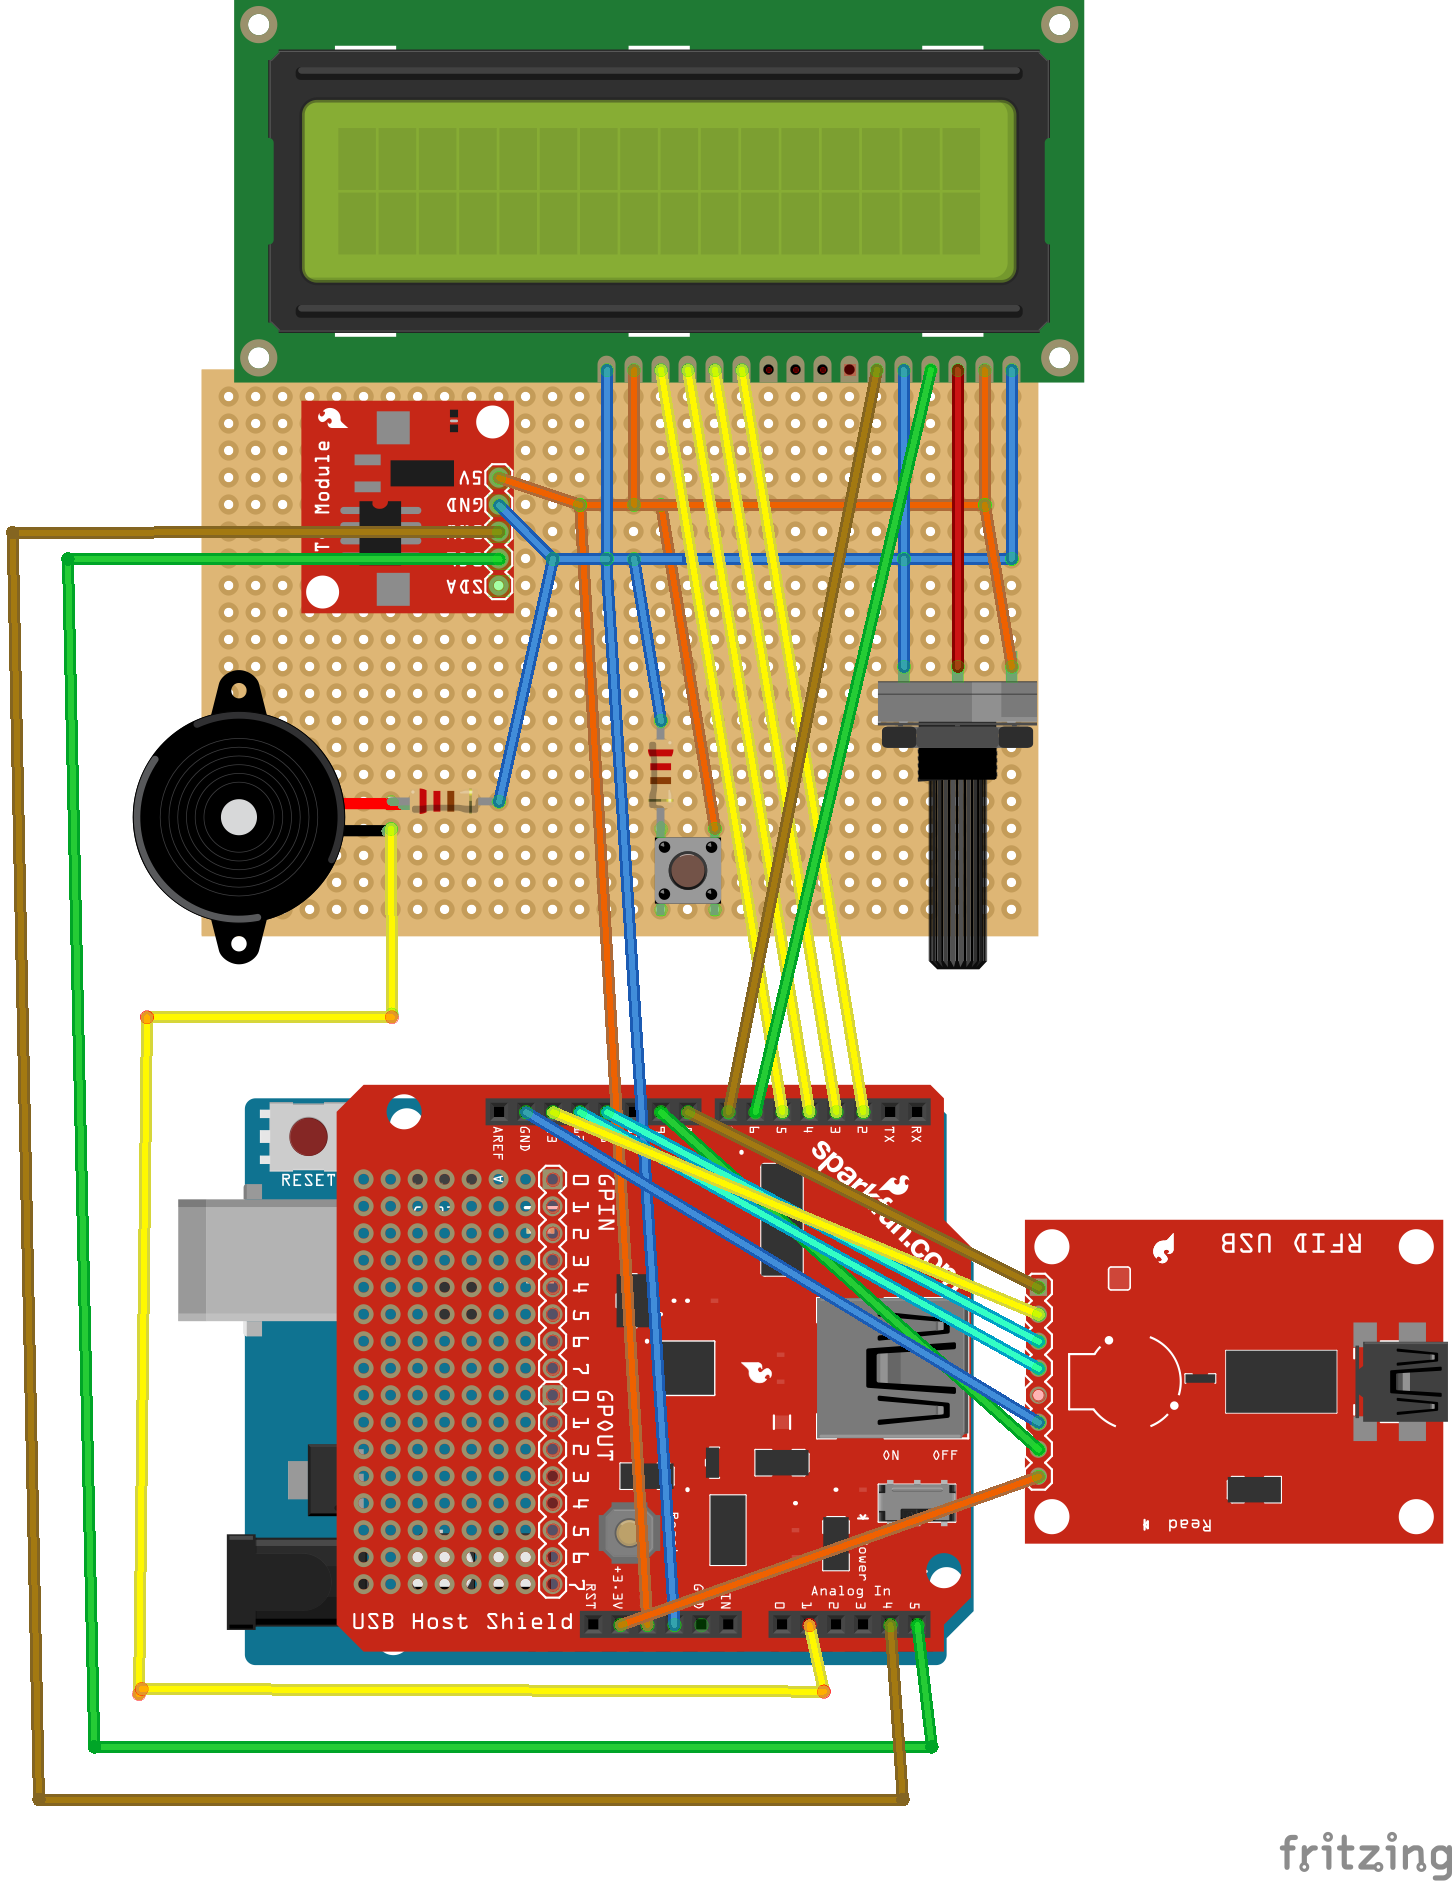
\includegraphics{circuit.png}
\end{figure}
\subsection{Działanie}
\indent Osią działania zaprojektowanego przeze mnie weryfikatora jest interakcja z dwoma zewnętrznymi urządzeniami. Jednym z nich jest nośnik danych na którym zapisane zostaną obecności uczesników zajęć jest w moim projektcie pendrive sformatowany w systemie FAT. W zależności od tego czy w danym momencie penrive jest podłączony, urządzenie jest w stanie oczekiwania na drugie z zewnętrznych narzędzie - elektroniczną legitymację studencką. Dodatkowo weryfikator jest zdolny do wyświetlanie komunikatów o swoim stanie na ekranie LCD i wydawania sygnałów dźwiękowych przy pomocy brzęczka. Cżęścią urządzenia jest również zegar RTC, który pozwala śledzić aktualną godzinę. Weryfikator monitoruje swój własny stan i jest zdolny do wykrywania błędów takich jak:
\begin{itemize}
\item Błąd inizjalizacji podłączonego pendriva
\item Błąd zapisu odczytanych danych na nośniku
\item Błąd zegara RTC - spowodowanego najczęściej rozładowaną baterią
\end{itemize}
\indent Kod mojego weryfikatora projektowałem z myślą o tym, żeby łatwo dało się przedstawić przebieg programu na diagramie. Strukura kodu jest przemyślana w taki sposób, żeby podczas jednego przebiegu pętli głównej wykonywał się jedynie kd powiazany z aktualnym stanem urządzenia. Taki układ nie tylko pozwala zwięźle opowiadać o działaniu urządzenia, ale również ulatwiał testowanie poprawności podczas pisania kodu i montowania urządzenia.
\indent Weryfikator w danej chwili może znajdować się w jednym z 12 stanów. Na przedstawionym diagramie stany oczekujące na zdarzenie przdstawiono kolorem kremowym, a stany przejściowe kolorem niebieskim:
\begin{figure}[h]
\caption{Diagram stanów}
\centering
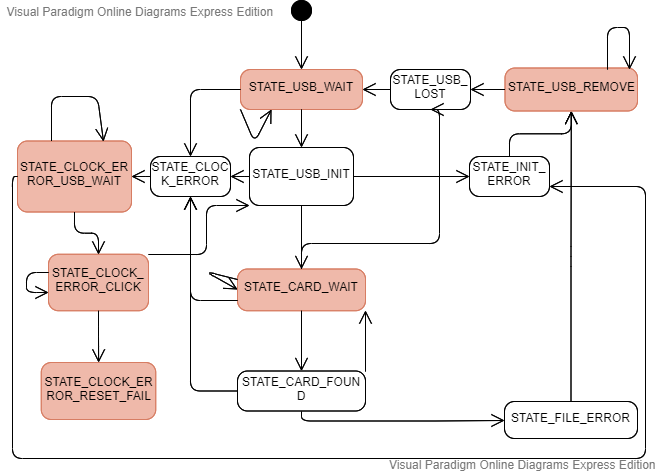
\includegraphics[scale=0.6]{state_machine.png}
\end{figure}

\begin{itemize}
\item STATE\_USB\_WAIT - czekanie na penrive - ekran wyświetla informację -  "Insert pendrive". Próba inicjalizacji nośnika zajmuje około 5 sekund dlatego wyświetlany czas jest aktualizowany z opóźnieniem
\item STATE\_USB\_INIT - inicjalizacja pendriva - po odnalezieniu pendriva wyświetlana jest informacja "USB Inserted". W przypadku błędu inicjalizacji - przejście do stanu STATE\_INIT\_ERROR,  w razie sukcesu na podstawie aktualnego czasu stworzona i zapiętana zostaje nazwa YY-MM-DD-hh\_mm\_ss dla pliku który będzie przechowywał zebrane uidy. STATE\_CARD\_WAIT w przeciwnym
\item STATE\_CARD\_WAIT - oczekiwanie na kartę RFID - ekran: "Scan Card". W razie wykrycia odłączenia penriva przejście do stanu STATE\_USB\_LOST. W przypadku wykrycia karty, ale błędu w odczycie (np. ze względu na zbyt szybkie odsunięcie karty) wyświetlenie informacji: Read error.
\item STATE\_CARD\_FOUND - zapisywanie Uidu do pliku - otwarcie pliku o zapamiętanej nazwie zapisanie do niego odczytanego Uidu. W razie błędu przy zapisie przejście do stanu STATE\_FILE\_ERROR, w przypadku sukcesu sygnał dźwiękowy, wyświetlenie informacji "Read Success" i powrót do stanu STATE\_CARD\_WAIT
\item STATE\_INIT\_ERROR - błąd inicjalizacji pendriva - ekran: "Init Error"
\item STATE\_USB\_REMOVE - czekanie na odłączenie pendriva. Wyświetlacz: "Reinsert USB". W razie wykrycia odłączenia penriva przejście do stanu STATE\_USB\_LOST.
\item STATE\_USB\_LOST - odłączono pendrive . Ekran: "USB removed", sygnał dźwiękowy oraz przejście do stanu STATE\_USB\_WAIT
\item STATE\_FILE\_ERROR - błąd zapisu do pliku. Ekran: "Open file error", przejście do stanu STATE\_USB\_REMOVE
\item STATE\_CLOCK\_ERROR  - błąd zegara - w razie wykrycia problemów z zegarem w którymś ze stanów [STATE\_USB\_WAIT, STATE\_CARD\_WAIT, STATE\_CARD\_FOUND, STATE\_USB\_INIT, STATE\_USB\_REMOVE] sterowanie przechodzi do tego stanu. Wyświetlona zostaje informacja: "Clock Error", następnie sterowanie przechodzi do STATE\_CLOCK\_ERROR\_USB\_WAIT
\item STATE\_CLOCK\_ERROR\_USB\_WAIT - oczekiwanie na pendrive z czasem - wyświetlacz "Insert pendrive with time". Sterowanie pozostaje w tym stanie do czasu kiedy na zewnętrznym nośniku wykryty zostanie plik o nazwie tdav, który w pierwszym wierszu będzie zawierał datę w formacie "YYYY/MM/DD hh:mm:ss". W przypadku wykrycia poprawnego pliku program zapamiętuje datę z pliku tdav i przechodzi w stan STATE\_CLOCK\_ERROR\_CLICK\\
- W razie błędu przy inicjalizacji pendriva program przechodzi do stanu STATE\_INIT\_ERROR \\
- W razie wykrycia pendrive i nie wykrycia pliku o nazwie tdav wyświetlona zostaje informacja "Upload time tdav"\\
- W razie złego formatu pierwszej linijki w pliku tdav wyświetlona zostaje informacja: "Bad date format"
\item STATE\_CLOCK\_ERROR\_CLICK - Czekanie na reset. Wyświetlacz: "Click to reset".  Sterowanie pozostaje w tym stanie do czasu kiedy zostanie przyciśnięty guzik resetu. Po naciśnięciu guzika na zegarze zostaje ustawiona zapamiętana data, wyświetlony zostaje komunikat "Time set", a sterowanie przechodzi w stan STATE\_USB\_INIT. Jeśli podczas ustawiania czasu na zagarze wystąpi błąd program przechodzi w stan STATE\_CLOCK\_ERROR\_RESET\_FAIL \\
\item STATE\_CLOCK\_ERROR\_RESET\_FAIL - błąd resetowania czasu. Wyświetlacz: "Clock Reset Fail". Ze względu na brak możliwośąciu ustawienia poprawnego czasu jest to stan ostatecznej porażki.
\end{itemize}
\subsection{Procedura resetowania zegara RTC}

\subsection{Napotkane problemy}
\subsubsection{Dwa moduły korzystające z interfejsu SPI}
\indent Początko zamiast Arduino Uno planowałem użyć innej wersji tej popularnej płytki - Arduino Leonardo. \\
\indent Tak jak w wersji którą ostatecznie zrealizowałem, planowałem do układu Leonardo podłączyć USB Host Shield oraz modułu RFID - oba używają intrfejsu SPI. Każdy z tych komponentów osobno współpracował poprawnie z Arduino Leonardo. Problemy pojawiły się kiedy próbwałem podłączyć wszystko w jedną całość i zapisywać odczytane dane z karty magnetycznej na podłączonym pendrivie. \\
\indent Podczas montowania ukladu problemem nie do przeskoczenia okazało się to, że w przypadku tej wersji płytki piny intefejsu SPI znajdują się w magistrali ICSP, która jest zajęta przez moduł USB w taki sposób, że nie ma możliwości podłączyć tam pinów inych pinów. \\
\indent Próbowałem jeszcze dolutować kable do magistrali CSP na płytce  USB Host Shield, jednak ze względu na to że, są to jedynie milimetrowe wypuski, przepaliłem któreś z połączeń wewnątrz tego układu i ostatecznie musiałem je wyrzucić. \\
W ostateczności przeszedłem na wersję UNO które interfejs SPI ma doprowadzony również na piny 10-13. Dodatkową modyfikajcą którą musiałem wprowadzić do układu było podłączenie pinu SS (slave select) modułu RFID do innego złącza niż 10, ponieważ był on już wykorzystywany przez USB Host Shield.
 \begin{figure}[h]
\caption{Uklad USB Host shield ze wskzaniem na zakończenia magistrali CSP}
\centering
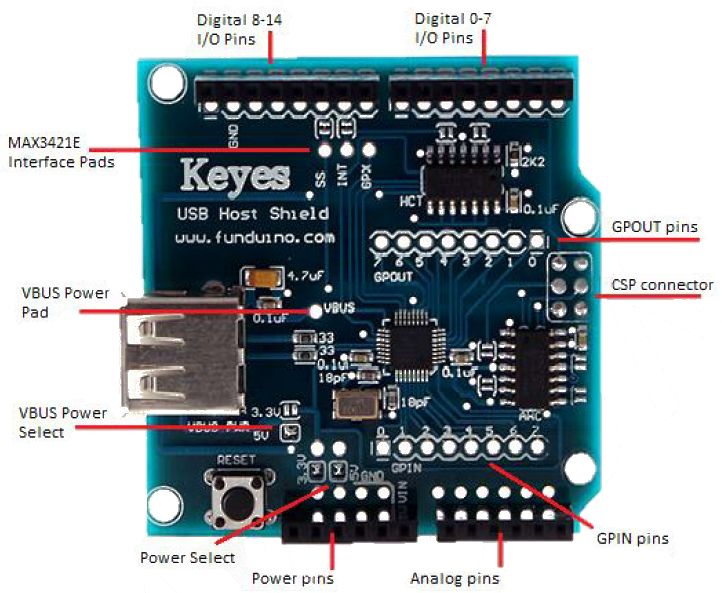
\includegraphics[scale=0.6]{usb_host_shield.jpg}
\end{figure}

\subsubsection{Wypełniona pamięć operacyjna}
\indent W miarę dołączania kolejnych komponentów do układu, tzn. zegara RTC, brzęczka oraz wyświetlacza LCD, zacząłem natrafiać na problemy z pamięcią. \\
\indent Pierwsza skończyła się pamięć operacyjna której mój kontroler posiadał jedynie 2KB. Objawiało się to nagłym zawieszaniem się wykonywania programu, co w pierwszym momencie było dla mnie zaskakujące i niezrozumiałe.
\indent Udało mi się rozwiązać ten problem dzięki większej dyscyplinie w korzystaniu z pamięci. Ograniczyłem liczbę zmiennych globalnych, a największy efekt przyniosło przeniesienie wykorzystywanych w programie napisów z pamięci operacyjnej do pamięci flash, do czego służy dyrektywa PROGMEM.
\indent Pamięć flash jest przeznaczona do przechwywania kodu programu i nie ma do niej swobodnego dostępu jak w przypadku pamięci operacyjnej. Dodanie kolejnej biblioteki która ułatwiłaby przechowywanie danych w tej przestrzeni nie było możliwym ze względu na graniczone zasoby.\\
\indent Ostatecznie zdecydowałem się na korzystanie z pamięci flash wczytując dane najt po bajcie. Chcąc więc wyświetlić komunikat na kranie LCD, tak czy inaczej musiałem najpierw wczytać bajtowo łańcuch znaków do pamięci operacyjnej, jednak nie było już potrzeby przechowywać wszystkich łańcuchów znaków jednocześnie w SRAM.
 \begin{figure}[h]
\caption{Stałe programu przechowywane w pamięci flash}
\centering
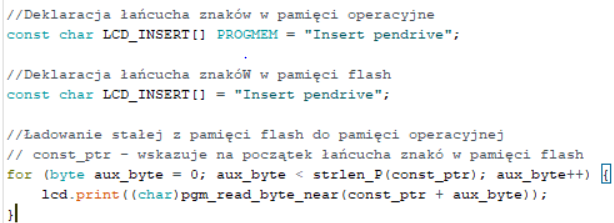
\includegraphics[scale=0.8]{progmem.png}
\end{figure}
\subsubsection{Wypełniona pamięć flash}
\indent Przeniesienie łańcuchów znaków do pamięci flash, chociaż poprawiło wydajność pamięci operacyjnej, to spowodowało wyczerpanie przestrzeni przeznaczonej  na kod programu. \\
\indent Pamięć flash jest bardziej pojemna niż SRAM ponieważ w tym wypadku jest to aż 32KB do dyspozycji programisty, jednak duża liczba bibliotek do obsługi peryferiów doprowadziła do wyczerpanie się również tej przestrzeni. \\
\indent Ułatwieniem w przypadku optymalizowania wykorzystania pamięci flash jest to, że przestrzeń zajmowana przez kod programu jest stała po kompilacji. Nie ma więc obawy że w trakcie przebiegu programu nastąpi nagły wzrost i przekroczenie pojemności. Wytraczy dostosować się do limitu 32 KB. \\
\indent Udało mi się tego dokonać poprzez ograniczenie liczby funkcji które deklarowałem w moim programie, oraz schowanie komunikatów wysyłanych na serial monitor wewnątrz dyrektyw preprocesora \#if DEBUG serial.println("SETUP"); \#endif. Dzięki temu mogłem łatwo wyłączyć kod programu odpowiedzialny za debugowanie.\\
\indent W pierszej wersji planowanego przeze mnie weryfikatora, miał on się łączyć z siecią za pomocą modułu WIFI. Bardzo dużo kłopotów sprawił mi jednak układ ESP8266, odpowiedzialny za tę łączność. Po wgraniu sterownika do tego układu przestawał on być wykrywany przez komputer i Arduino\\. \indent Pomimo wykorzystania kilku takich układów za każdym razem ojawiał się ten sam problem  Nie udało mi się dociec jaka była tego przyczyna. Ostatecznie odszedłem od wykorzytania modułu ESP8266 ze względu na zmianę koncepcji.
\subsection{Inne koncepcje}
\indent Zastanawiając się nad ostateczną formą jaką powinien przyjąć projektowany przeze mnie weryfikator brałem jeszcze pod uwagę układ Rosberry Pi. Ostatecznie zrezygnowałem z tego pomysłu, ze względu na to ża takie urządzenie mogłoby wymagać utrzymywania systemu operacyjnego aktualnej wersji. Za wykorzystaniem Arduino przemawiała również cena takiego układu i fakt, że jest on mi bardzo dobrze znany z zajęć Systemów Wbudowanych.\\
\indent Projektując układ usiałem również podjąć decyzję z jakiego nośnika skorzystać do przenoszenia danych z weryfikatora do aplikacji zarządzającejobecnosciami. Brałem pod uwagę dwie możliwości. Poza opcją na którą się ostatecznie zdecydowałem, brałem jeszcze pod uwagę korzystanie z kart SD \\
\indent Ze względu na większą dostępnąść i łatwiejsze podłączenie klasycznego pendriva do komputera ( nie każdy komputer posiada slot na kartę SD), zdecydowałem się nie tę właśnie możliwość.  Później okazało się, że ta decyzja miała swoje konsekwncje.\\
\indent Po pierwsze USB Host Shield zajął magistralę ICSP, będącą jedynym wyjściem pinów interfejsu SPI w układzie Arduino Leonrado. Po perypetiach wcześniej już przeze mnie opisanych, zdecydowałem się na zmianę wersji płytki na Uno. \\
\indent Kolejnym utrudnieniem które zostało postawione na mojej drodze ze względu na korzystanie z pendriva, były problemy z dostępnością biblioteki obsługującej pamięć w tej formie. Podstawowa biblioteka obslugująca układ USB Host Shield nie przwiduje wykorzystania złącza USB do podłączenia pamięci masowej. \\
\indent Ostatecznie udało mi się znaleźć nieszczególnie popularną bibliotekę do obsługi tego narzędzia - UsbFat, która jednak okazała się być słabo opisana.
\section{Menadżer obecności - umożliwiający katalogowanie daych}
\section{Baza studentów - umożliwiająca identyfikakację danych zebranych z ELS}

\chapter{Możliwości rozwoju}
\begin{itemize}
\item dostęp do usos i propagowanie zebranych danych na stronach uczelnianych
\item Udostępnienie systemu dla studentów i umożliwienie monitorowania swoich obecności (logowanie tylko przez uczelnianego maila, albo konta utworzone wyłącznie przez administratora)
\item powiadomienia mailowe do studenta o zbliżającym się wyczerpaniu limitu nieobecności
\end{itemize}

\chapter{Wnioski}

\ldots

%%%%% BIBLIOGRAFIA

%\begin{thebibliography}{1}
%\bibitem{example} \ldots
%\end{thebibliography}

\end{document}


